\documentclass{article}
\usepackage[dblblindworkshop]{neurips_2026}
\workshoptitle{AgenticOS @ NeurIPS 2026}

\usepackage[utf8]{inputenc}
\usepackage[T1]{fontenc}
\usepackage{hyperref}
\usepackage{url}
\usepackage{booktabs}
\usepackage{amsfonts}
\usepackage{amsmath}
\usepackage{nicefrac}
\usepackage{microtype}
\usepackage{xcolor}
\usepackage{graphicx}
\usepackage{enumitem}

\newcommand{\hal}{\textsc{hal}}
\newcommand{\rhoS}{\rho}

\title{Does Cost-Efficiency Travel?\
Rank Transfer and Frontier Stability in Fixed-Scaffold Agent Evaluation}
\author{Anonymous Author(s)}

\begin{document}
\maketitle

\begin{abstract}
Agent leaderboards increasingly report task success and dollar cost, inviting practitioners to select a ``cost-efficient'' system from a single benchmark. We test whether this signal transfers across workloads. Using public Holistic Agent Leaderboard (\hal) results, we hold the displayed HAL Generalist Agent scaffold fixed and compare repeated displayed model labels across six benchmarks. Several high-overlap pairs exhibit robust positive transfer in both accuracy and dollar-cost ranks: among pairs with at least 12 shared labels, cost Spearman correlation ranges from $0.74$ to $0.93$, survives Holm--Bonferroni correction, and exceeds a label-permutation null. Across all pairs, negative cost estimates occur only at low overlap ($N\leq9$), have configuration-resampling intervals crossing zero, and do not survive multiplicity or permutation checks. Cost--accuracy frontier membership is nevertheless non-universal: no label tested on at least five workloads lies on every frontier under nondominance, a HAL-inspired convex hull, or a 5\% near-tie sensitivity. A single leaderboard can therefore provide a useful prior but not a universal efficiency guarantee.
\end{abstract}

\section{Introduction}

Agent benchmarks evaluate systems that reason over multiple steps, invoke tools, and interact with environments. Reported behavior depends on the language model, scaffold, tools, prompts, execution limits, and task environment. Evaluation is also expensive: \hal{} reports 21,730 rollouts across nine benchmarks and roughly \$40,000 in cost~\citep{kapoor2026hal}. Cost-aware leaderboards therefore plot accuracy against dollar cost and recommend cost--accuracy frontiers.

A practical question follows: if a displayed model label is efficient on one agent benchmark, is it a promising low-cost choice elsewhere? This may hold when capability and resource use are portable, but can fail when tool calls, retries, or stopping behavior differ by environment. We study this question descriptively, holding the publicly displayed HAL Generalist Agent scaffold fixed and matching exact public model-label strings across workloads.

Our design is coverage-aware. Most HAL scaffolds occur on only one benchmark, making a global model--scaffold decomposition unsupported. The Generalist Agent is the only broadly repeated scaffold. We retain six benchmarks with adequate pairwise overlap and analyze accuracy rank, dollar-cost rank, and frontier membership only among shared labels. Our contributions are:
\begin{itemize}[leftmargin=*,nosep]
    \item A cross-workload analysis that distinguishes robust high-overlap evidence from low-overlap descriptive estimates.
    \item Configuration-resampling, Holm-corrected, and label-permutation checks for pairwise rank associations.
    \item A frontier sensitivity analysis separating nondominance, a HAL-inspired randomized-policy hull, and a conservative near-tie tolerance.
\end{itemize}

The result is neither universal transfer nor universal non-transfer. Several high-overlap pairs show robust positive accuracy- and cost-rank transfer; sparse low-overlap pairs are too uncertain to establish either transfer or reversal. No broadly tested label is a universal cost--accuracy frontier winner.

\section{Related work}

\paragraph{Cost-aware agent evaluation.}
\citet{kapoor2026hal} introduce HAL as a standardized, cost-aware leaderboard across coding, web, science, and customer-service tasks, with dollar- and token-cost frontiers and scaffold comparisons. \citet{agentsmatter2024} argue for joint accuracy--cost evaluation of agents. SWE-Effi studies resource-constrained software-engineering agents and reports scaffold--model interaction within one domain~\citep{sweeffi2025}. These works motivate cost-aware evaluation but do not measure cross-workload rank transfer under a repeated scaffold.

\paragraph{Ranking stability.}
\citet{ndzomga2026efficient} ask whether reduced task subsets preserve \emph{within-benchmark} agent rankings under scaffold and temporal shift. Benchmark$^2$ evaluates cross-benchmark ranking consistency for static LLM benchmarks~\citep{qian2026benchmark2}. We adapt rank consistency to interactive agents and separately examine accuracy, dollar cost, and cost--accuracy frontiers.

\section{Data and method}
\label{sec:method}

We analyze the public \texttt{all\_leaderboards\_costs\_HAL.csv} snapshot distributed with \citet{ndzomga2026efficient}: 242 displayed evaluations across nine benchmarks, 11 displayed scaffolds, and 29 displayed model labels. Accuracy and total dollar cost are complete; 235 rows report one run and only seven report two. The frozen source, hash, and code are documented in the anonymous supplement.

The primary cohort fixes the displayed HAL Generalist Agent scaffold. It contains 21 labels on CORE-Bench Hard, 17 on GAIA, 9 on SciCode, 7 on ScienceAgentBench, 18 on SWE-bench Verified Mini, and 14 on TAU-bench Airline. USACO has one Generalist result and is excluded. Figure~\ref{fig:coverage} shows the incomplete coverage.

\begin{figure}[t]
  \centering
  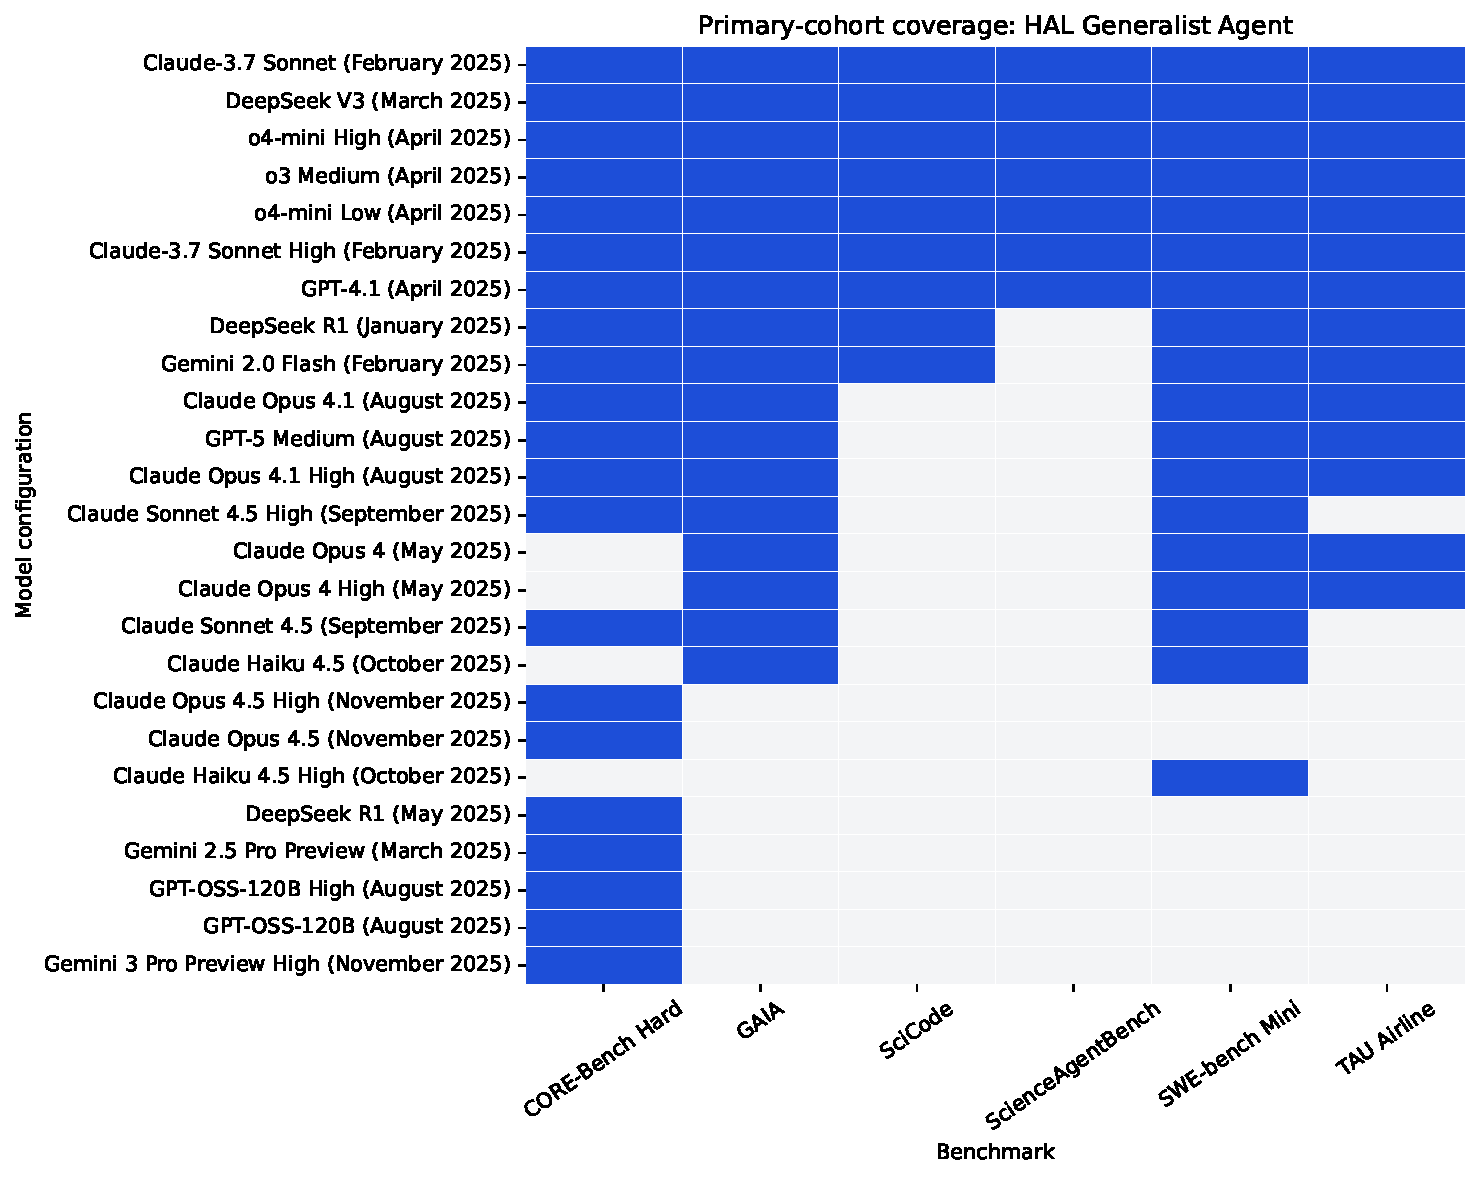
\includegraphics[width=0.94\linewidth]{figures/coverage_heatmap.pdf}
  \caption{Primary-cohort coverage. A filled cell denotes a public HAL row for that displayed label under the displayed Generalist scaffold.}
  \label{fig:coverage}
\end{figure}

For each pair with at least five shared labels, we compute Spearman $\rhoS$ and Kendall rank correlation separately for accuracy and dollar cost. We use 10,000 configuration-resampling draws to characterize sensitivity to the finite shared-label set. These are not rollout-level or population-model confidence intervals. We also permute pairing between observed rank vectors 10,000 times to form a finite-$N$ null and apply Holm--Bonferroni correction separately to 15 accuracy and 15 cost tests.

For lower cost and higher accuracy, a nondominated point has no competitor that is at least as accurate and no more costly with one strict improvement. We additionally implement a HAL-inspired origin-anchored convex-hull reconstruction, which permits a randomized-policy interpretation, and a 5\% tolerance sensitivity where dominance requires both 5\% lower cost and 5\% higher accuracy. The tolerance is a near-tie stress test, not a calibrated measurement-error model.

\section{Results}

\subsection{Robust rank transfer is concentrated in high-overlap pairs}

Figure~\ref{fig:similarity} shows all point estimates. The strongest evidence comes from the six pairs with at least 12 shared labels. GAIA--SWE-mini has 17 shared labels and correlations $\rhoS=0.71$ for accuracy and $0.89$ for cost. SWE-mini--TAU has $\rhoS=0.76$ and $0.82$. All six high-overlap positive cost associations survive Holm correction and the label-permutation null.

Low-overlap negative cost estimates do not support a reversal claim. For example, GAIA--ScienceAgentBench has cost $\rhoS=-0.75$ over seven labels, but its configuration-resampling interval is [-1.00, 0.17], it does not survive Holm correction, and its permutation $p=0.0675$. We report this as an indeterminate sparse-pair estimate rather than evidence of negative transfer.

\begin{figure*}[t]
  \centering
  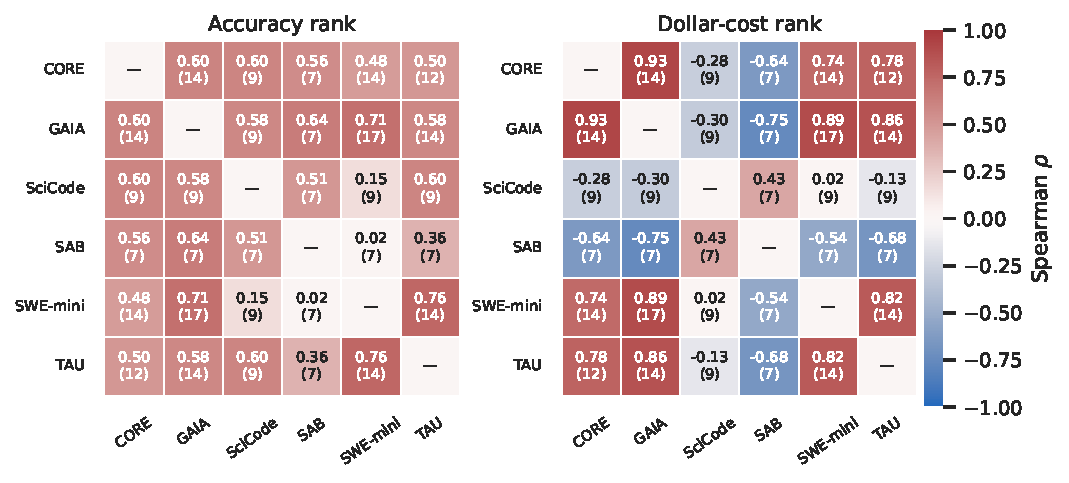
\includegraphics[width=0.98\textwidth]{figures/rank_transfer_compact.pdf}
  \caption{Cross-workload rank-transfer point estimates under the displayed HAL Generalist Agent scaffold. Each cell reports Spearman $\rhoS$ and the number of shared labels. Main-text claims rely on high-overlap pairs; complete robustness results are in the supplement.}
  \label{fig:similarity}
\end{figure*}

\begin{table}[t]
\caption{Higher-overlap pairs. Brackets are configuration-resampling sensitivity intervals; ND is nondominated-frontier Jaccard similarity on the shared-label cohort.}
\label{tab:highoverlap}
\centering
\footnotesize
\begin{tabular}{lrrrr}
\toprule
Pair & N & Accuracy $\rho$ & Cost $\rho$ & ND Jaccard \\
\midrule
CORE-Bench Hard--GAIA & 14 & 0.60 [0.16, 0.81] & 0.93 [0.72, 0.99] & 0.43 \\
CORE-Bench Hard--SWE-bench Mini & 14 & 0.48 [-0.05, 0.82] & 0.74 [0.29, 0.93] & 0.25 \\
CORE-Bench Hard--TAU Airline & 12 & 0.50 [-0.12, 0.86] & 0.78 [0.26, 0.98] & 0.17 \\
GAIA--SWE-bench Mini & 17 & 0.71 [0.31, 0.91] & 0.89 [0.61, 0.99] & 0.33 \\
GAIA--TAU Airline & 14 & 0.58 [0.14, 0.85] & 0.86 [0.58, 0.97] & 0.29 \\
SWE-bench Mini--TAU Airline & 14 & 0.76 [0.40, 0.91] & 0.82 [0.46, 0.97] & 0.43 \\
\bottomrule
\end{tabular}

\end{table}

\subsection{Frontier membership is non-universal}

Figure~\ref{fig:frontier} shows nondominated membership. No label tested on at least five workloads is nondominated on every workload. This conclusion survives all three frontier definitions: nondominance, the HAL-inspired hull, and 5\% near-tie tolerance. The stronger statement that no label appears on more than 4/6 frontiers does not survive: under tolerance, o4-mini Low appears on 5/6. We therefore retain only the non-universal-winner conclusion.

\begin{figure}[t]
  \centering
  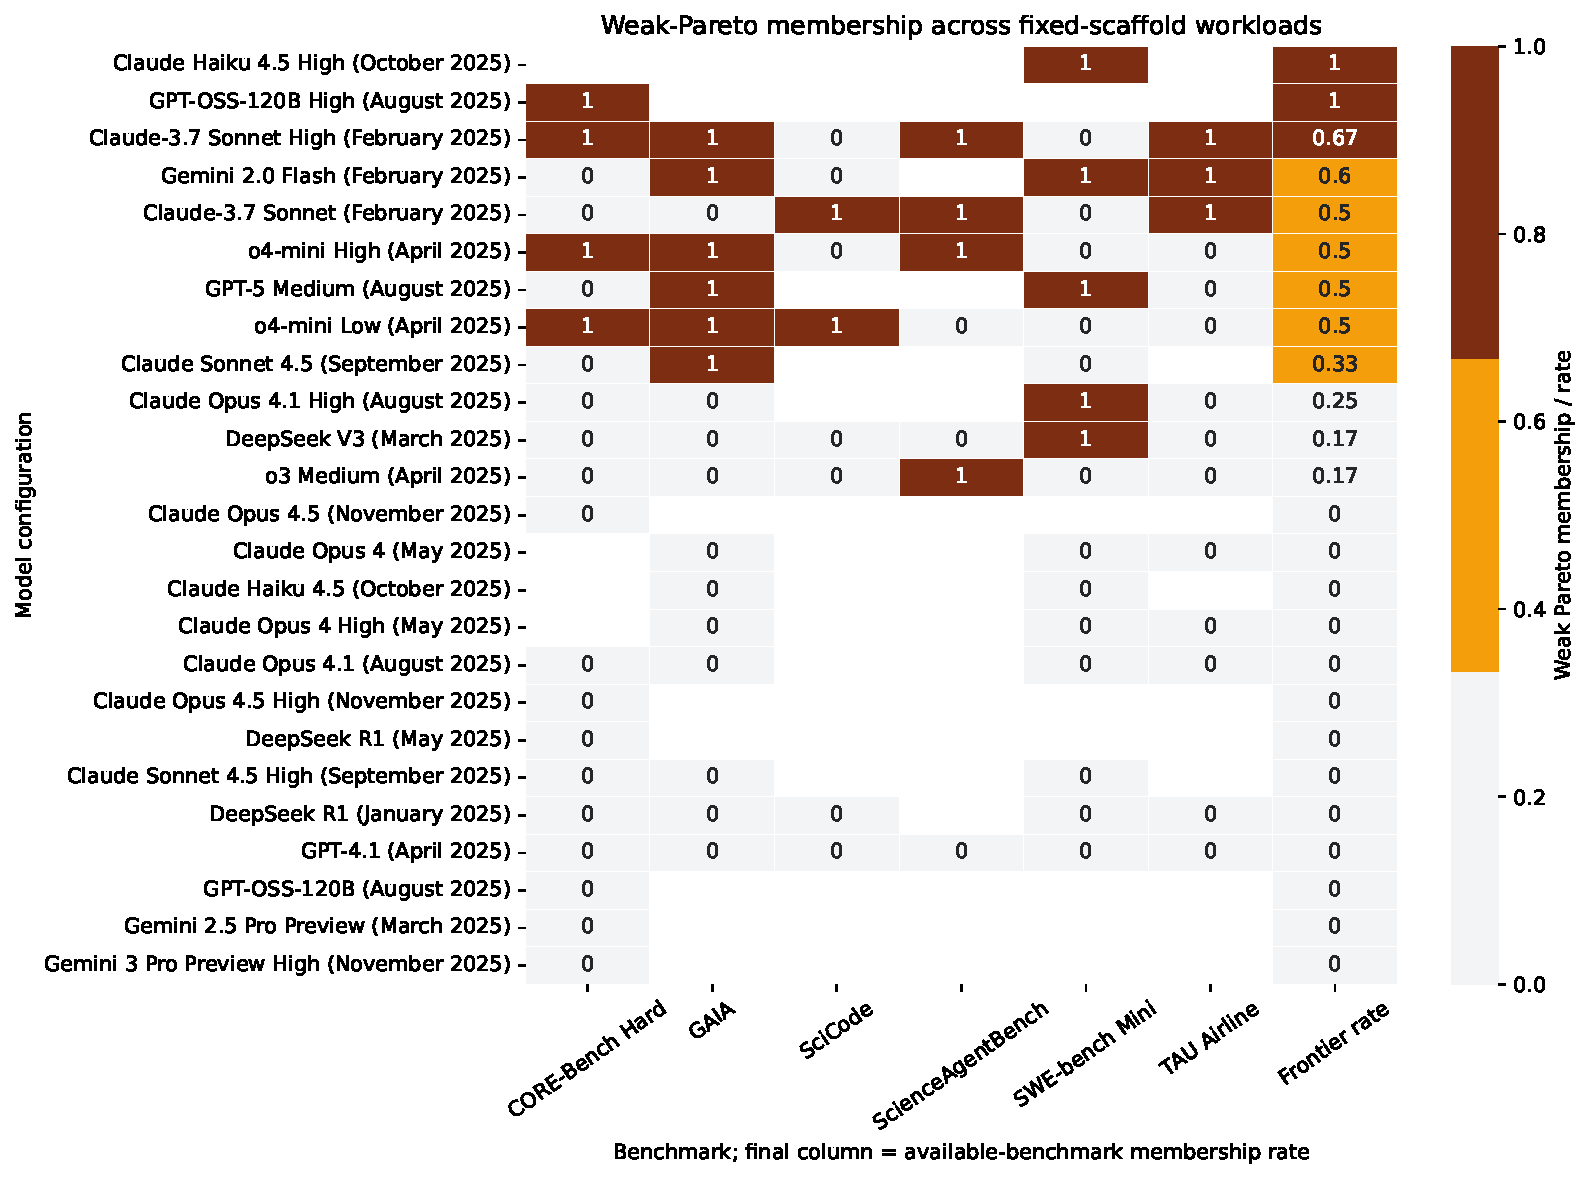
\includegraphics[width=0.98\linewidth]{figures/weak_pareto_membership.pdf}
  \caption{Nondominated cost--accuracy membership across primary workloads. The final column is each label's rate over available workloads. No broadly tested label appears on every available frontier.}
  \label{fig:frontier}
\end{figure}

\begin{table}[t]
\caption{Nondominated frontier appearances for labels tested on at least five workloads.}
\label{tab:rates}
\centering
\footnotesize
\begin{tabular}{lrrr}
\toprule
Model label & Tested & ND appearances & ND rate \\
\midrule
Claude-3.7 Sonnet High & 6 & 4 & 0.67 \\
Claude-3.7 Sonnet & 6 & 3 & 0.50 \\
o4-mini High & 6 & 3 & 0.50 \\
o4-mini Low & 6 & 3 & 0.50 \\
DeepSeek V3 & 6 & 1 & 0.17 \\
o3 Medium & 6 & 1 & 0.17 \\
GPT-4.1 & 6 & 0 & 0.00 \\
Gemini 2.0 Flash & 5 & 3 & 0.60 \\
DeepSeek R1 & 5 & 0 & 0.00 \\
\bottomrule
\end{tabular}

\end{table}

\subsection{Scaffold and frontier definitions matter}

The source HAL labels recover 30 rows under the hull reconstruction, with two discrepancies; ordinary nondominance includes 19 additional points. A discrete buyer choosing one system and a deployer willing to randomize between systems therefore face different decision frontiers.

Within individual benchmarks, scaffolds also differ substantially. Across 15 shared labels on SWE-mini, the displayed SWE-Agent averages 27.4 percentage points higher accuracy than the Generalist scaffold, with higher median cost. Across seven shared labels on ScienceAgentBench, SAB Self-Debug is both more accurate on average and lower cost. These contrasts motivate fixing the scaffold; they are not a general causal scaffold estimate.

\section{Discussion and threats to validity}

A single benchmark can supply a useful cost-selection prior, and several high-overlap pairs show robust positive cost-rank transfer. It does not guarantee transfer to every workload: sparse pairs are indeterminate, and no broad label is universally on the cost--accuracy frontier. Practitioners should validate cost on representative target tasks rather than treating one leaderboard frontier as universal.

Construct validity is limited because public \texttt{Models} and \texttt{Agent Name} strings do not fully encode prompts, tools, budgets, harness versions, or pricing assumptions. Matching a display label under the Generalist scaffold is not a controlled base-model comparison. Internal validity is limited by sparse, unbalanced coverage and mostly single-run evaluations. DeepSeek R1 and Gemini 2.0 Flash are absent from ScienceAgentBench, but the public table provides no failure or exclusion reason; missingness is unidentifiable rather than assumed random. Dollar cost also combines execution behavior and contemporary price assumptions, while the supplied CSV lacks total-token columns. External validity is restricted to this frozen HAL snapshot and six workloads.

\section{Conclusion}

Several high-overlap public HAL workload pairs show robust positive accuracy- and dollar-cost-rank transfer under a repeated displayed Generalist scaffold. Sparse low-overlap comparisons are too uncertain to establish reversals. Cost--accuracy frontier membership is non-universal under multiple decision-frontier definitions. A leaderboard can provide a useful prior, but not a universal efficiency guarantee.

\bibliographystyle{plainnat}
\bibliography{references}

\clearpage
\appendix
\section{Supplementary robustness results}

\begin{table*}[t]
\caption{All pairwise Spearman correlations and 10,000-draw configuration-resampling sensitivity intervals.}
\centering
\scriptsize
\begin{tabular}{lrrr}
\toprule
Pair & N & Acc. $\rho$ [interval] & Cost $\rho$ [interval] \\
\midrule
CORE-Bench Hard--GAIA & 14 & 0.60 [0.16, 0.81] & 0.93 [0.72, 0.99] \\
CORE-Bench Hard--SciCode & 9 & 0.60 [-0.24, 0.92] & -0.28 [-0.86, 0.51] \\
CORE-Bench Hard--ScienceAgentBench & 7 & 0.56 [-0.41, 1.00] & -0.64 [-1.00, 0.17] \\
CORE-Bench Hard--SWE-bench Mini & 14 & 0.48 [-0.04, 0.82] & 0.74 [0.27, 0.93] \\
CORE-Bench Hard--TAU Airline & 12 & 0.50 [-0.11, 0.85] & 0.78 [0.26, 0.98] \\
GAIA--SciCode & 9 & 0.58 [-0.19, 0.98] & -0.30 [-0.89, 0.55] \\
GAIA--ScienceAgentBench & 7 & 0.64 [-0.18, 1.00] & -0.75 [-1.00, 0.17] \\
GAIA--SWE-bench Mini & 17 & 0.71 [0.32, 0.91] & 0.89 [0.60, 0.99] \\
GAIA--TAU Airline & 14 & 0.58 [0.16, 0.85] & 0.86 [0.57, 0.97] \\
SciCode--ScienceAgentBench & 7 & 0.51 [-0.64, 1.00] & 0.43 [-0.62, 1.00] \\
SciCode--SWE-bench Mini & 9 & 0.15 [-0.66, 0.78] & 0.02 [-0.81, 0.81] \\
SciCode--TAU Airline & 9 & 0.60 [0.00, 0.92] & -0.13 [-0.80, 0.76] \\
ScienceAgentBench--SWE-bench Mini & 7 & 0.02 [-0.97, 0.65] & -0.54 [-1.00, 0.65] \\
ScienceAgentBench--TAU Airline & 7 & 0.36 [-0.76, 0.96] & -0.68 [-1.00, 0.19] \\
SWE-bench Mini--TAU Airline & 14 & 0.76 [0.41, 0.91] & 0.82 [0.46, 0.97] \\
\bottomrule
\end{tabular}

\end{table*}

\begin{table*}[t]
\caption{Holm--Bonferroni results, corrected separately within 15 accuracy and 15 cost tests.}
\centering
\scriptsize
\begin{tabular}{llrrc}
\toprule
Pair & Metric & Uncorrected p & Holm p & Reject \\
\midrule
corebench\_hard--gaia & Accuracy & 0.0222 & 0.2891 & No \\
corebench\_hard--scicode & Accuracy & 0.0903 & 0.9328 & No \\
corebench\_hard--scienceagentbench & Accuracy & 0.1925 & 0.9623 & No \\
corebench\_hard--swebench\_verified\_mini & Accuracy & 0.0848 & 0.9328 & No \\
corebench\_hard--taubench\_airline & Accuracy & 0.0965 & 0.9328 & No \\
gaia--scicode & Accuracy & 0.1012 & 0.9328 & No \\
gaia--scienceagentbench & Accuracy & 0.1194 & 0.9328 & No \\
gaia--swebench\_verified\_mini & Accuracy & 0.0015 & 0.0222 & Yes \\
gaia--taubench\_airline & Accuracy & 0.0294 & 0.3524 & No \\
scicode--scienceagentbench & Accuracy & 0.2474 & 0.9898 & No \\
scicode--swebench\_verified\_mini & Accuracy & 0.6992 & 1.0000 & No \\
scicode--taubench\_airline & Accuracy & 0.0886 & 0.9328 & No \\
scienceagentbench--swebench\_verified\_mini & Accuracy & 0.9694 & 1.0000 & No \\
scienceagentbench--taubench\_airline & Accuracy & 0.4271 & 1.0000 & No \\
swebench\_verified\_mini--taubench\_airline & Accuracy & 0.0017 & 0.0238 & Yes \\
corebench\_hard--gaia & Cost & 0.0000 & 0.0000 & Yes \\
corebench\_hard--scicode & Cost & 0.4600 & 1.0000 & No \\
corebench\_hard--scienceagentbench & Cost & 0.1194 & 0.8357 & No \\
corebench\_hard--swebench\_verified\_mini & Cost & 0.0027 & 0.0294 & Yes \\
corebench\_hard--taubench\_airline & Cost & 0.0030 & 0.0299 & Yes \\
gaia--scicode & Cost & 0.4328 & 1.0000 & No \\
gaia--scienceagentbench & Cost & 0.0522 & 0.4696 & No \\
gaia--swebench\_verified\_mini & Cost & 0.0000 & 0.0000 & Yes \\
gaia--taubench\_airline & Cost & 0.0001 & 0.0009 & Yes \\
scicode--scienceagentbench & Cost & 0.3374 & 1.0000 & No \\
scicode--swebench\_verified\_mini & Cost & 0.9661 & 1.0000 & No \\
scicode--taubench\_airline & Cost & 0.7324 & 1.0000 & No \\
scienceagentbench--swebench\_verified\_mini & Cost & 0.2152 & 1.0000 & No \\
scienceagentbench--taubench\_airline & Cost & 0.0938 & 0.7500 & No \\
swebench\_verified\_mini--taubench\_airline & Cost & 0.0003 & 0.0035 & Yes \\
\bottomrule
\end{tabular}

\end{table*}

\begin{table}[t]
\caption{Cost-quartile flips in shared-label pairs.}
\centering
\scriptsize
\begin{tabular}{lrrr}
\toprule
Pair & N & Cheap-to-expensive & Any extreme flip \\
\midrule
corebench\_hard--gaia & 14 & 0/14 (0\%) & 0/14 (0\%) \\
corebench\_hard--scicode & 9 & 1/9 (11\%) & 2/9 (22\%) \\
corebench\_hard--scienceagentbench & 7 & 1/7 (14\%) & 2/7 (29\%) \\
corebench\_hard--swebench\_verified\_mini & 14 & 1/14 (7\%) & 1/14 (7\%) \\
corebench\_hard--taubench\_airline & 12 & 0/12 (0\%) & 0/12 (0\%) \\
gaia--scicode & 9 & 1/9 (11\%) & 3/9 (33\%) \\
gaia--scienceagentbench & 7 & 1/7 (14\%) & 3/7 (43\%) \\
gaia--swebench\_verified\_mini & 17 & 0/17 (0\%) & 0/17 (0\%) \\
gaia--taubench\_airline & 14 & 0/14 (0\%) & 0/14 (0\%) \\
scicode--scienceagentbench & 7 & 0/7 (0\%) & 0/7 (0\%) \\
scicode--swebench\_verified\_mini & 9 & 2/9 (22\%) & 3/9 (33\%) \\
scicode--taubench\_airline & 9 & 2/9 (22\%) & 3/9 (33\%) \\
scienceagentbench--swebench\_verified\_mini & 7 & 2/7 (29\%) & 3/7 (43\%) \\
scienceagentbench--taubench\_airline & 7 & 2/7 (29\%) & 2/7 (29\%) \\
swebench\_verified\_mini--taubench\_airline & 14 & 0/14 (0\%) & 0/14 (0\%) \\
\bottomrule
\end{tabular}

\end{table}

\begin{table}[t]
\caption{Universal-winner sensitivity to frontier definition. Broad labels are tested on at least five workloads.}
\centering
\scriptsize
\begin{tabular}{lrc}
\toprule
Definition & Max appearances (broad labels) & Universal broad winner \\
\midrule
Nondominated & 4 & No \\
HAL-inspired hull & 3 & No \\
Nondominated, 5\% tolerance & 5 & No \\
\bottomrule
\end{tabular}

\end{table}

\begin{figure*}[t]
  \centering
  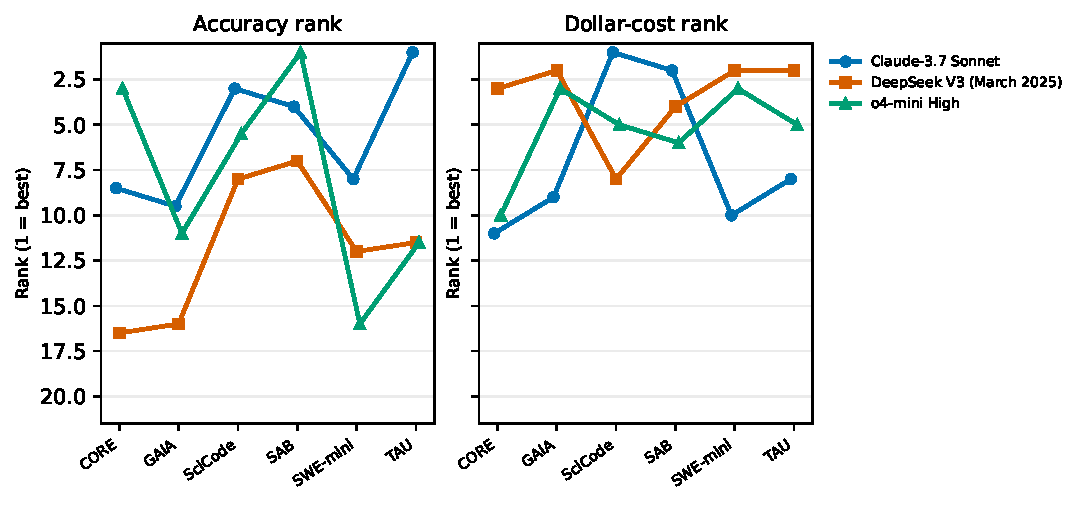
\includegraphics[width=0.78\textwidth]{figures/rank_change_slopegraph.pdf}
  \caption{Supplementary rank-line view for three labels observed on all six primary workloads. Ranks are among all displayed Generalist labels available on each benchmark; lower is better. Ties use average ranks; markers are slightly offset only to keep tied series visible.}
\end{figure*}

\section{Frontier-label reproducibility audit}
\begin{table}[h]
\caption{Supplied HAL frontier labels compared with reconstructed frontiers.}
\centering
\scriptsize
\begin{tabular}{lrrrrrr}
\toprule
Benchmark & Rows & Supplied & Nondominated & Hull & Supplied--ND agreement & Supplied--hull agreement \\
\midrule
assistantbench & 15 & 2 & 3 & 2 & 0.933 & 1.000 \\
corebench\_hard & 45 & 5 & 10 & 5 & 0.889 & 1.000 \\
gaia & 32 & 4 & 6 & 4 & 0.938 & 1.000 \\
online\_mind2web & 22 & 3 & 4 & 3 & 0.955 & 1.000 \\
scicode & 33 & 2 & 3 & 3 & 0.970 & 0.970 \\
scienceagentbench & 23 & 4 & 8 & 4 & 0.826 & 1.000 \\
swebench\_verified\_mini & 33 & 3 & 7 & 3 & 0.879 & 1.000 \\
taubench\_airline & 26 & 3 & 3 & 4 & 1.000 & 0.962 \\
usaco & 13 & 4 & 5 & 4 & 0.923 & 1.000 \\
\bottomrule
\end{tabular}

\end{table}

\section{Reproducibility details}
The anonymous supplement contains the frozen source hash, public data provenance, source code, generated tables, tests, and commands. The primary analysis uses exact public display labels, minimum overlap five, 10,000 configuration-resampling draws, 10,000 null permutations, and fixed seed 20260816.

\section*{NeurIPS Paper Checklist}

\begin{enumerate}
\item \textbf{Claims}
    \item[] Question: Do the main claims made in the abstract and introduction accurately reflect the paper's contributions and scope?
    \item[] Answer: \answerYes{}
    \item[] Justification: The abstract and introduction state that the analysis is descriptive, restricted to repeated public HAL display labels under a repeated displayed scaffold, and does not identify causal model or scaffold effects.

\item \textbf{Limitations}
    \item[] Question: Does the paper discuss the limitations of the work performed by the authors?
    \item[] Answer: \answerYes{}
    \item[] Justification: Section~6 discusses sparse coverage, display-label ambiguity, single-run evaluations, price dependence, missing token totals, limited domain comparisons, and frontier sensitivity.

\item \textbf{Theory assumptions and proofs}
    \item[] Question: For each theoretical result, does the paper provide the full set of assumptions and a complete (and correct) proof?
    \item[] Answer: \answerNA{}
    \item[] Justification: The paper presents an empirical secondary analysis and no theoretical results.

\item \textbf{Experimental result reproducibility}
    \item[] Question: Does the paper fully disclose all the information needed to reproduce the main experimental results of the paper to the extent that it affects the main claims and/or conclusions of the paper (regardless of whether the code and data are provided or not)?
    \item[] Answer: \answerYes{}
    \item[] Justification: Sections~3--4 and the appendix specify the public source, frozen hash, inclusion criteria, matching unit, frontier definitions, overlap threshold, resampling procedure, and seed.

\item \textbf{Open access to data and code}
    \item[] Question: Does the paper provide open access to the data and code, with sufficient instructions to faithfully reproduce the main experimental results, as described in supplemental material?
    \item[] Answer: \answerYes{}
    \item[] Justification: An anonymized supplement will contain the analysis code, provenance manifest, and reproduction instructions; the underlying public data source is cited.

\item \textbf{Experimental setting/details}
    \item[] Question: Does the paper specify all the training and test details (e.g., data splits, hyperparameters, how they were chosen, type of optimizer) necessary to understand the results?
    \item[] Answer: \answerYes{}
    \item[] Justification: No models are trained. The data filtering, rank metrics, frontier definitions, resampling count, and seed are specified in Sections~3--4.

\item \textbf{Experiment statistical significance}
    \item[] Question: Does the paper report error bars suitably and correctly defined or other appropriate information about the statistical significance of the experiments?
    \item[] Answer: \answerYes{}
    \item[] Justification: We report configuration-resampling sensitivity intervals and explicitly state that they are not rollout-level or population-model confidence intervals and are not used for hypothesis tests.

\item \textbf{Experiments compute resources}
    \item[] Question: For each experiment, does the paper provide sufficient information on the computer resources (type of compute workers, memory, time of execution) needed to reproduce the experiments?
    \item[] Answer: \answerNA{}
    \item[] Justification: The work is a lightweight secondary analysis of public tabular data and uses no model training or agent rollouts.

\item \textbf{Code of ethics}
    \item[] Question: Does the research conducted in the paper conform, in every respect, with the NeurIPS Code of Ethics \url{https://neurips.cc/public/EthicsGuidelines}?
    \item[] Answer: \answerYes{}
    \item[] Justification: The work uses public aggregate evaluation data, attributes source authors, reports limitations, and makes no claims about people or protected groups.

\item \textbf{Broader impacts}
    \item[] Question: Does the paper discuss both potential positive societal impacts and negative societal impacts of the work performed?
    \item[] Answer: \answerYes{}
    \item[] Justification: We use **Yes** here because the work has practical consequences. Better reporting of success-adjusted cost and execution telemetry can reduce wasted evaluation and deployment spend. Conversely, treating a single leaderboard's dollar ranking as a deployment recommendation can misallocate resources or favor systems whose price/configuration signal does not transfer. The paper's safeguards are explicit claim boundaries, public-data provenance, and reproducible sensitivity analyses.

\item \textbf{Safeguards}
    \item[] Question: Does the paper describe safeguards that have been put in place for responsible release of data or models that have a high risk for misuse (e.g., pre-trained language models, image generators, or scraped datasets)?
    \item[] Answer: \answerNA{}
    \item[] Justification: The paper releases no trained model, agent capability, or new high-risk dataset.

\item \textbf{Licenses for existing assets}
    \item[] Question: Are the creators or original owners of assets (e.g., code, data, models), used in the paper, properly credited and are the license and terms of use explicitly mentioned and properly respected?
    \item[] Answer: \answerYes{}
    \item[] Justification: The data and methodological sources are cited; the supplement records the upstream repository, commit, source path, and declared MIT license.

\item \textbf{New assets}
    \item[] Question: Are new assets introduced in the paper well documented and is the documentation provided alongside the assets?
    \item[] Answer: \answerYes{}
    \item[] Justification: The analysis code and generated tables are documented by a source manifest, artifact manifest, tests, and reproduction commands.

\item \textbf{Crowdsourcing and research with human subjects}
    \item[] Question: For crowdsourcing experiments and research with human subjects, does the paper include the full text of instructions given to participants and screenshots, if applicable, as well as details about compensation (if any)?
    \item[] Answer: \answerNA{}
    \item[] Justification: The study involves no crowdsourcing and no human subjects research.

\item \textbf{Institutional review board (IRB) approvals or equivalent for research with human subjects}
    \item[] Question: Does the paper describe potential risks incurred by study participants, whether such risks were disclosed to the subjects, and whether Institutional Review Board (IRB) approvals (or an equivalent approval/review based on the requirements of your country or institution) were obtained?
    \item[] Answer: \answerNA{}
    \item[] Justification: The study involves no human subjects research.

\item \textbf{Declaration of LLM usage}
    \item[] Question: Does the paper describe the usage of LLMs if it is an important, original, or non-standard component of the core methods in this research?
    \item[] Answer: \answerNA{}
    \item[] Justification: The core method is deterministic analysis of public tabular data; no LLM is used as a component of the empirical method.
\end{enumerate}

\end{document}
